\chapter{Existing methods of detecting breast cancer}
\label{chap:ch2}



\textcolor{green}{eu as face cateva modificari:\\
1. titlu - as zice "problem definition and existing methods of detecting breast cancer in images"\\
2. as include o sectiune dedicata prezentarii problemei:\\
- ce se da (o imagine) 
- ce se cere (un label --- normal, malign, benign ---, un bounding-box in jurul tumorii)
- cum stim ca AI/ML-ul rezolva bine problema - adica ce metrici putem folosi (acc, prec, recall, IoU, etc.)\\
si abia apoi as veni cu o sectiune care sa descrie cele 3 seturi de date (cele care acum sunt in sectiunile 4.1 si 4.2) si apoi o sectiune de "related work"}

\par There are several articles related to studying various ways of implementing breast cancer detection using machine learning. There is “Machine Learning Techniques for Breast Cancer Prediction” by Varsha Nemade and Vishal Fegade from Mukesh Patel School of Technology Management and Engineering, NMIMS Shirpur Campus, India~\cite{carte2}. They have documented different ML classification techniques and evaluated each of them using different performance measures, such as accuracy, precision, and recall. These techniques include N{\"a}ive Bayes, Logistic Regression, Support Vector Machine, K-Nearest Neighbour and Decision Tree, the latter being found to have the highest accuracy, 97\%. 
\textcolor{green}{ar fi util sa spui cate clase au folosit si care au fost ele}

The dataset used in their experiments was the WDBC dataset, which contains features from 569 digitized images of a fine needle aspirate of a breast mass~\cite{link3}. The algorithm implemented uses features from the image rather than the image itself, some of which include radius, texture, area, perimeter, smoothness, compactness, concavity, concavity points, symmetry and fractal dimension. The following charts represent the performance of the classification techniques used.

\begin{figure}[h!]
    \centering
    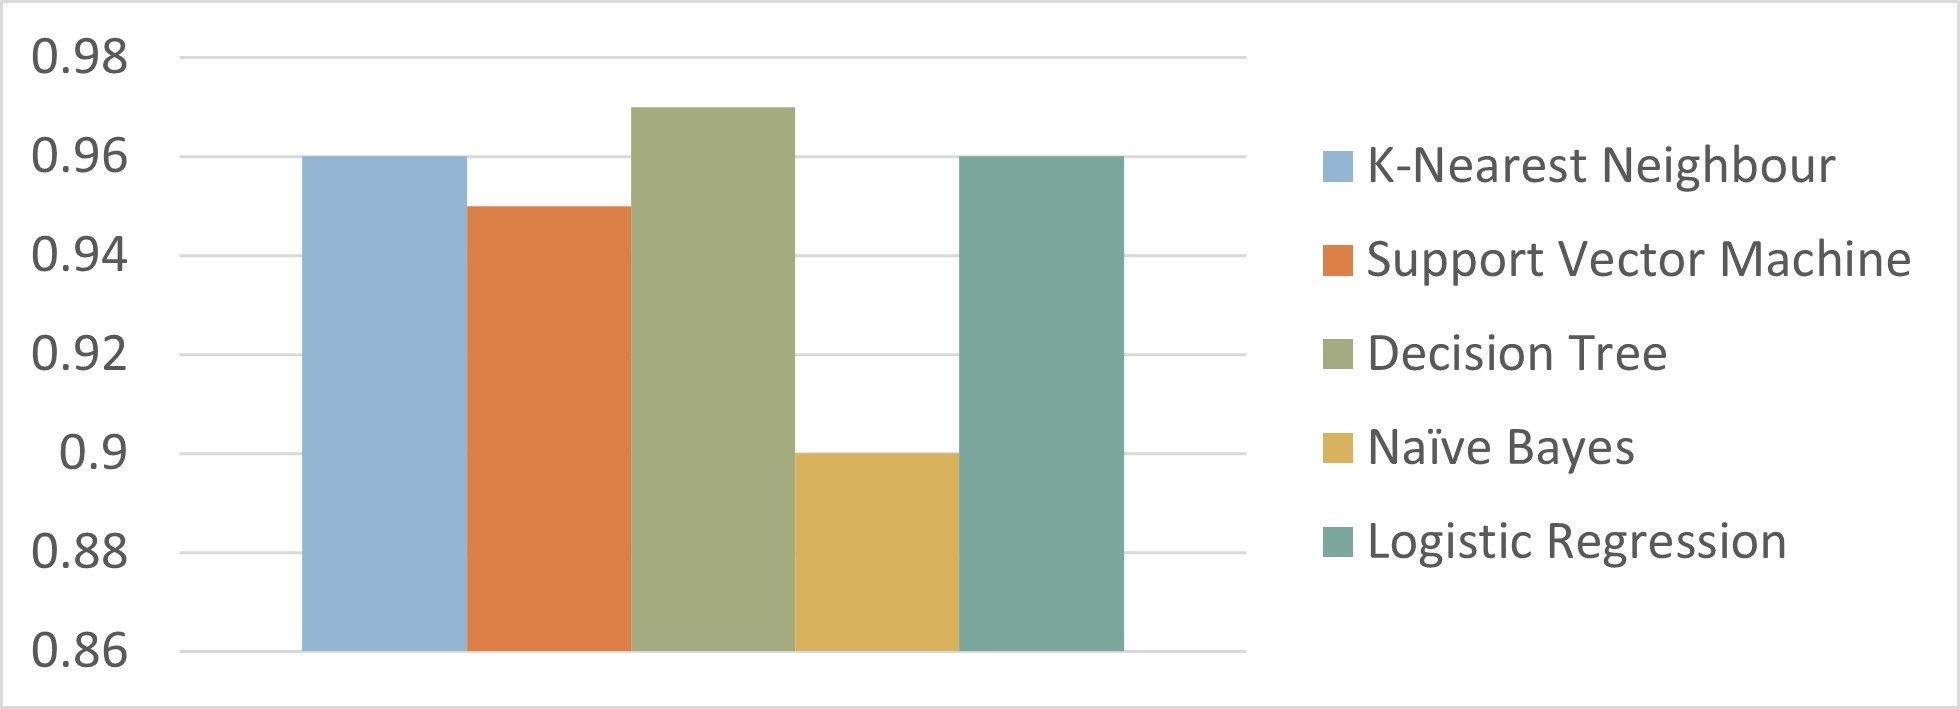
\includegraphics[width=0.75\textwidth]{figures/Figure1.jpg}
    \caption{Accuracy of classification techniques obtained in ~\cite{carte2}}
    \label{fig:fig1}
\end{figure}
\begin{figure}[h!]
    \centering
    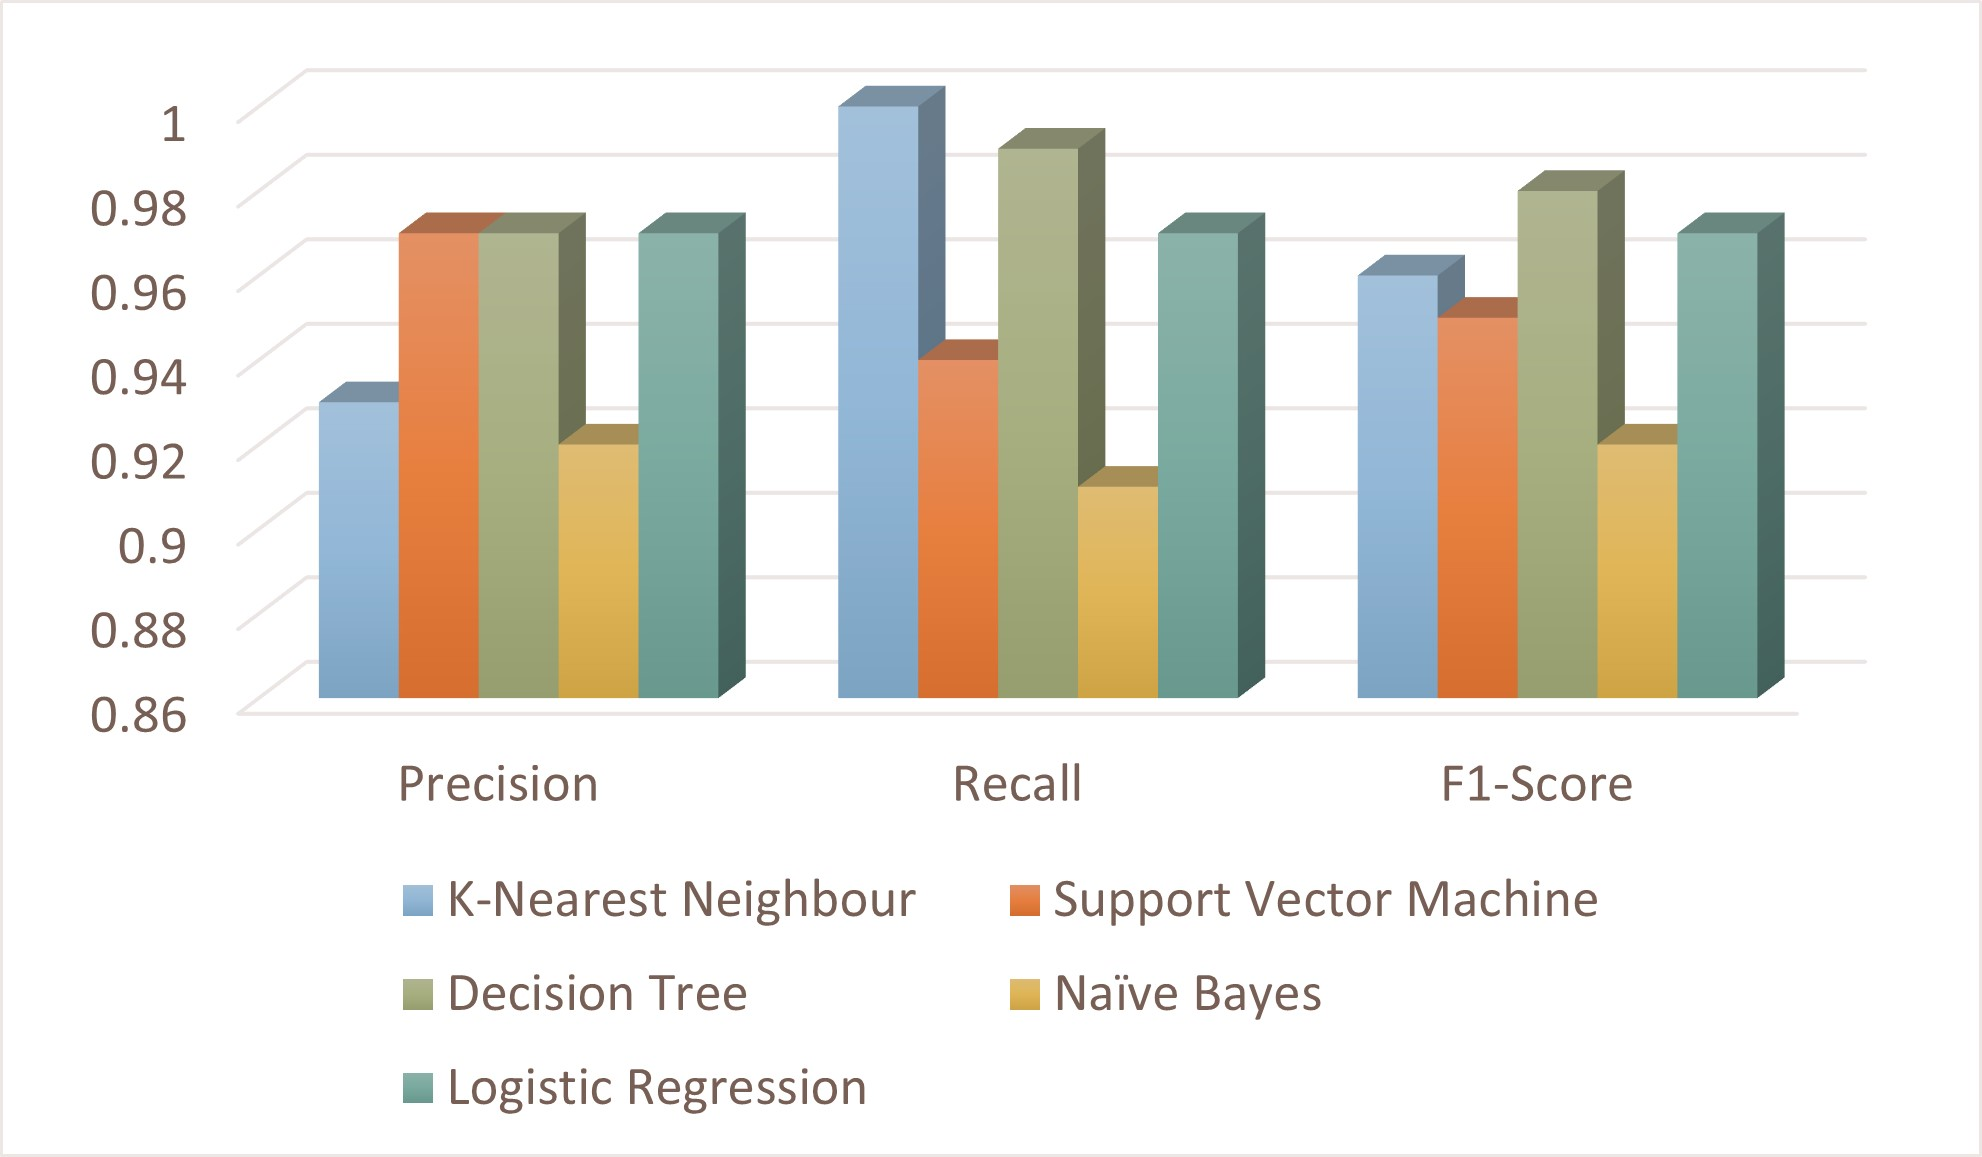
\includegraphics[width=0.75\textwidth]{figures/Figure2.jpg}
    \caption{Performance of classification techniques for class benign
    \textcolor{green}{sa spui si in care paper s-au obtinut aceste rezultate (e suficient sa adaugi citarea - vezi \ref{fig:fig1})}
    }
    \label{fig:fig2}
\end{figure}
\begin{figure}[h!]
    \centering
    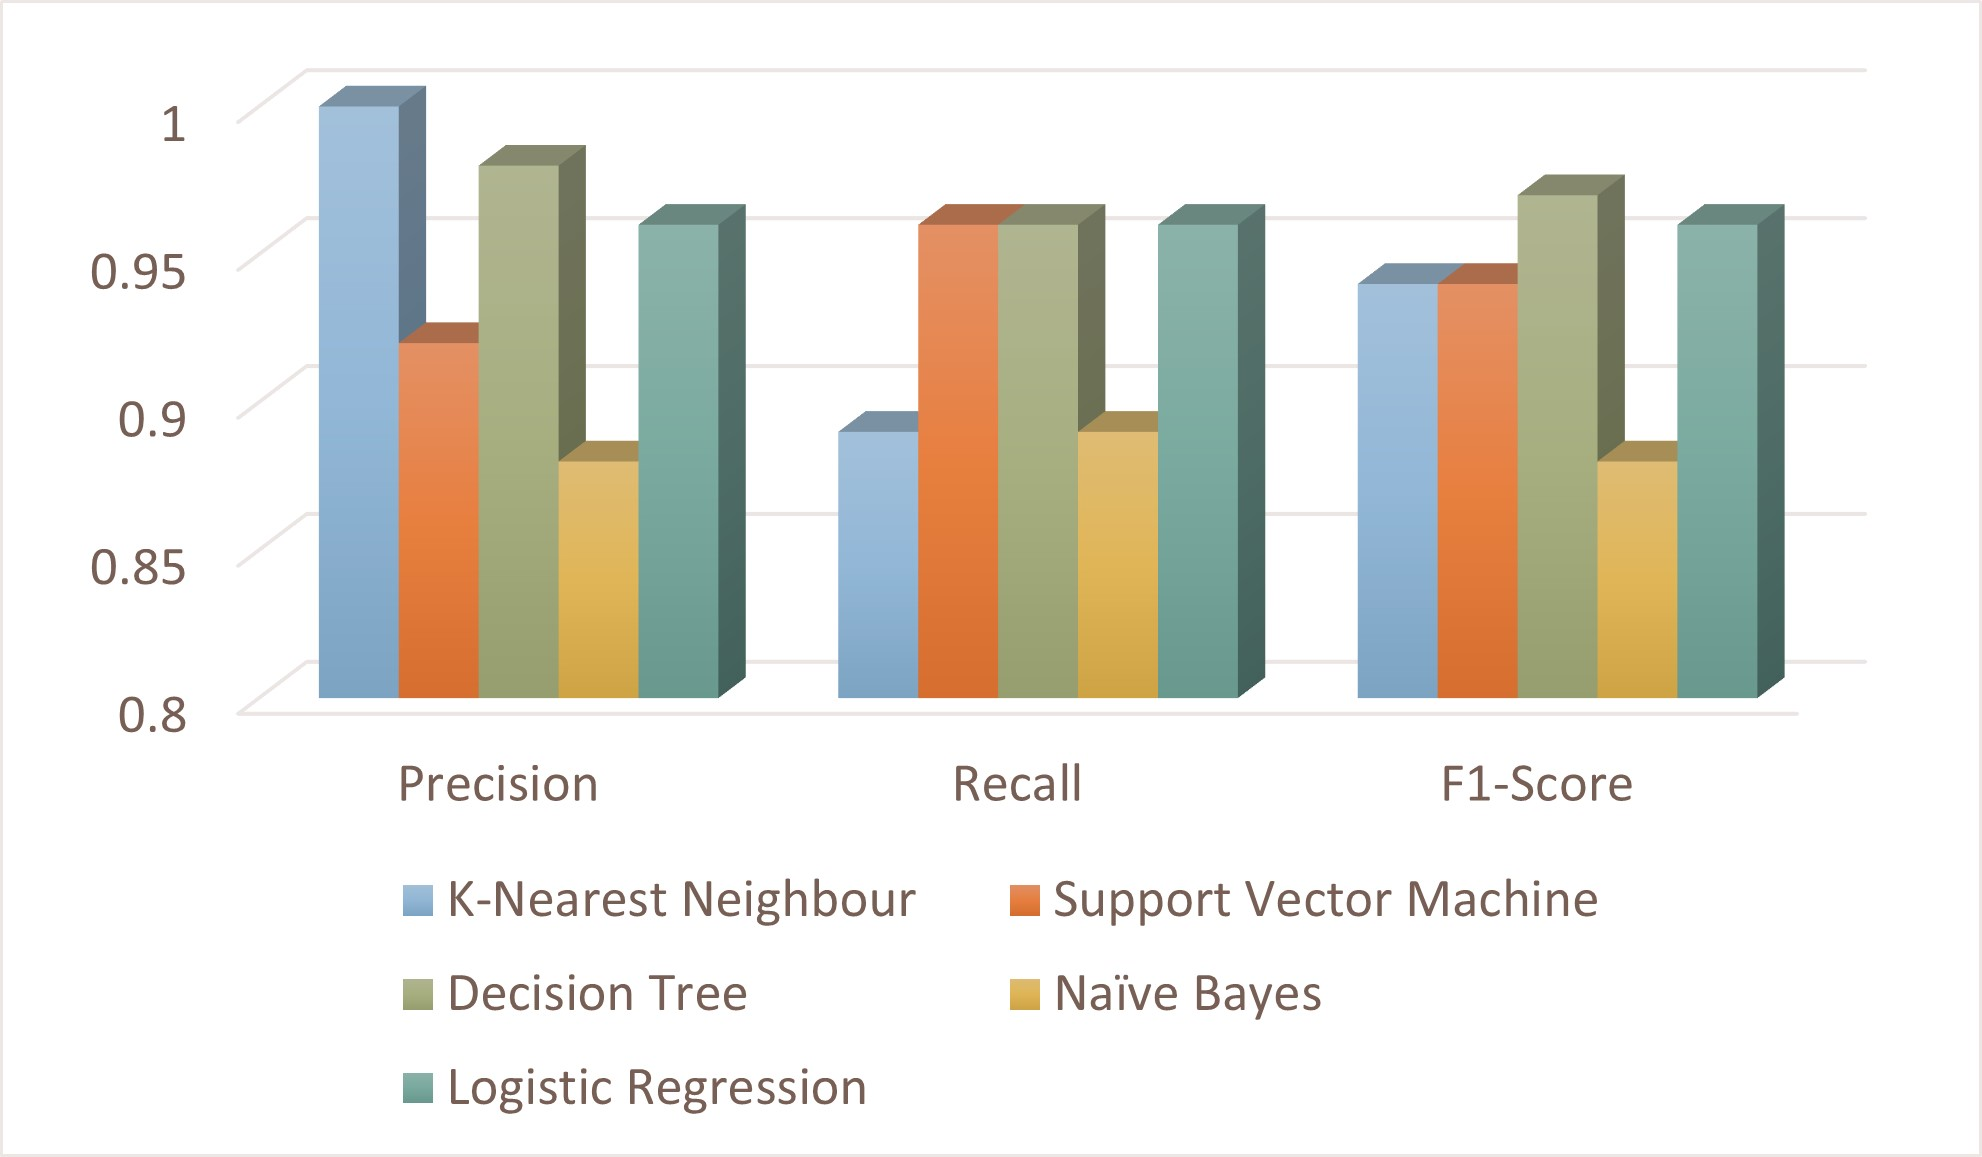
\includegraphics[width=0.75\textwidth]{figures/Figure3.jpg}
    \caption{Performance of classification techniques for class malignant
    \textcolor{green}{sa spui si in care paper s-au obtinut aceste rezultate (e suficient sa adaugi citarea - vezi \ref{fig:fig1})}
    }
    \label{fig:fig3}
\end{figure}

Other relevant studies include “An enhanced Predictive heterogeneous ensemble model for breast cancer prediction” concluded by S. Nanglia et al. which got 78\% accuracy using KNN, SVM and DT~\cite{carte1}. Islam et al. got a 98.75\% using ANN on the WDBC~\cite{carte3}. Amrane et al. proposed an approach using KNN and NB with 97.51\% accuracy~\cite{carte4}. Dhahri et al. studied the usage of genetic programming techniques for the selection of the best features and parameters for the machine learning classifier~\cite{carte5}.